\documentclass[3p]{elsarticle} %review=doublespace preprint=single 5p=2 column
%%% Begin My package additions %%%%%%%%%%%%%%%%%%%

\usepackage[hyphens]{url}


\usepackage{lineno} % add
  \linenumbers % turns line numbering on

\usepackage{graphicx}
%%%%%%%%%%%%%%%% end my additions to header

\usepackage[T1]{fontenc}
\usepackage{lmodern}
\usepackage{amssymb,amsmath}
\usepackage{ifxetex,ifluatex}
\usepackage{fixltx2e} % provides \textsubscript
% use upquote if available, for straight quotes in verbatim environments
\IfFileExists{upquote.sty}{\usepackage{upquote}}{}
\ifnum 0\ifxetex 1\fi\ifluatex 1\fi=0 % if pdftex
  \usepackage[utf8]{inputenc}
\else % if luatex or xelatex
  \usepackage{fontspec}
  \ifxetex
    \usepackage{xltxtra,xunicode}
  \fi
  \defaultfontfeatures{Mapping=tex-text,Scale=MatchLowercase}
  \newcommand{\euro}{€}
\fi
% use microtype if available
\IfFileExists{microtype.sty}{\usepackage{microtype}}{}
\usepackage[]{natbib}
\bibliographystyle{plainnat}

\ifxetex
  \usepackage[setpagesize=false, % page size defined by xetex
              unicode=false, % unicode breaks when used with xetex
              xetex]{hyperref}
\else
  \usepackage[unicode=true]{hyperref}
\fi
\hypersetup{breaklinks=true,
            bookmarks=true,
            pdfauthor={},
            pdftitle={Temnothorax rugatulus ants do not change their nest walls in response to environmental humidity},
            colorlinks=false,
            urlcolor=blue,
            linkcolor=magenta,
            pdfborder={0 0 0}}

\setcounter{secnumdepth}{0}
% Pandoc toggle for numbering sections (defaults to be off)
\setcounter{secnumdepth}{0}


% tightlist command for lists without linebreak
\providecommand{\tightlist}{%
  \setlength{\itemsep}{0pt}\setlength{\parskip}{0pt}}




\usepackage{parskip}

\begin{document}


\begin{frontmatter}

  \title{\emph{Temnothorax rugatulus} ants do not change their nest
walls in response to environmental humidity}
    \author[a]{Greg T. Chism}
   \ead{gchism@arizona.edu} 
    \author[b]{Wiley Faron}
  
    \author[c]{Anna Dornhaus}
  
      \affiliation[a]{Graduate Interdisciplinary Program in Entomology
and Insect Science, University of Arizona, Tucson, AZ, U.S.A.}
    \affiliation[b]{Department of Molecular and Cellular Biology,
University of Arizona, Tucson, AZ, U.S.A.}
    \affiliation[c]{Department of Ecology and Evolutionary Biology,
University of Arizona, Tucson, AZ, U.S.A.}
    \cortext[cor1]{Corresponding author}
  
  \begin{abstract}
  Animal architectures are interesting biological phenomena that can
  greatly increase the fitness of the builder and exist in a variety of
  forms and functions across taxa. Among the most intricate
  architectures are social insect nests, which may have several
  functions, one of which is the control of internal microclimate. In
  social insects, the regulation particularly of humidity in the nest
  can be crucial for the survival and growth of the brood. Though much
  is known on how nest excavating social insects respond to
  environmental humidity, little is known about how ants that build on
  to pre-existing cavities respond. Here we use the rock ant
  \emph{Temnothorax rugatulus} to determine whether and how colonies
  respond to environmental humidity by building and changing their nest
  architectures in pre-existing nest spaces. We specifically test the
  hypothesis that \emph{T. rugatulus} colonies build different nest
  walls, e.g.~wider or denser ones, in response to lower environmental
  humidity. We allowed \emph{T. rugatulus} colonies to build nest walls
  with two substrates across a 0-100\% relative humidity gradient. We
  further compare the porosity - empty volume in built nest walls - of
  natural \emph{T. rugatulus} nest walls with these artificial building
  substrates and the substrate compositions of built walls from our
  experiment. We found that humidity did not influence the nest walls
  \emph{T. rugatulus} colonies built in our experiment, concluding that
  regulating humidity is likely not a key function of \emph{T.
  rugatulus} nest wall architecture. We also found that the porosities
  of the artificial substrate that was predominantly used by the ants in
  our experiment were like the porosity of natural \emph{T. rugatulus}
  nest walls, indicating that ants had constant preferences for
  particular substrates. Physical nest wall features, including
  porosity, are therefore unlikely to be flexibly regulated in response
  to external humidity, but may be adaptations in other ways.
  \end{abstract}
    \begin{keyword}
    Ants \sep Nest Architecture \sep Temnothorax \sep Humidity \sep 
    Nest Building
  \end{keyword}
  
 \end{frontmatter}

\newpage

\hypertarget{introduction}{%
\section{Introduction}\label{introduction}}

Ants are some of the most ecologically diverse and evolutionarily
successful organisms {[}1{]} likely at least in part due to the
existence of nests that span in complexity from simple one-chambered
spaces to complex spaces with several dozen chambers {[}2--8{]}. Nests
serve as a stable and defensible space that likely facilitated the
development of the social lifestyle and reproductive division of labor,
i.e.~a separation between reproducing individuals and non-reproducing
`workers' {[}1, 9{]}. Due to this intimate tie to their nest, social
insect colonies have been referred to as a `factory within a fortress'
{[}9{]}.

~

Many social insects modify their nests to respond to different
environmental conditions to control their microclimate {[}10{]}.
Regulating humidity for example has been shown to be a key role in the
nest architecture in some social insects, such as leaf cutter ants, in
which workers plug nest holes to prevent desiccation {[}11, 12{]} and
mound building termites which construct a sophisticated nest ventilation
system that constantly changes throughout the day {[}13-15{]} Humidity
is particularly relevant to ants since larvae and eggs desiccate in dry
conditions {[}16-18{]}. Though we know much about how humidity
influences social insect colonies such as the above that excavate their
nests by removing substrate from the ground, the effect of the abiotic
environment on social insect colonies that build nests by adding
material, such as walls in rock crevices (additive nest builders), are
not well studied.

~

\emph{Temnothorax rugatulus} ants are found in pine and juniper zones in
northern Mexico, the western United States and southwestern Canada, and
have a colony size between 50 to 400 ants {[}19{]}. They reside in
preexisting structures such as rock crevices and acorns (i.e.~arboreal
and hypogaeic), thus creating a dark, cool, and humid nest space.
Members of the \emph{Temnothorax} genus are additive builders that
utilize stones (i.e.~what might, at this scale, be called sand grains)
and other environmental substrates to produce walls that change their
occupied nest space {[}20-21{]}. \emph{Temnothorax} colonies choose a
smaller-grained substrate when carrying is less energetically expensive
(e.g.~placed closer to the nest) {[}22-23{]}, but larger stones are
preferred during nest expansion and contraction {[}24{]}, possibly
because of the need for speed in building. \emph{Temnothorax rugatulus}
colonies both build thicker walls when they have more brood, and build
longer, larger area walls in higher environmental humidity {[}25{]}.
However, in that study, colonies were only offered one grain type. Walls
built with two stone sizes that are well mixed produce a higher angle
stability and thus are more structurally stable, because smaller grains
can fill in the gaps of larger grains {[}23{]}. We propose that mixed
walls may also regulate nest microclimate more efficiently than single
substrate walls by creating a more compact structure.

~

In this study we asked whether the ant \emph{Temnothorax rugatulus}
produces different nest walls in response to differing environmental
humidity. Response to humidity is reasonable since \emph{T. rugatulus}
colonies live inside crevices found in granite boulders in a desert
environment that likely experience occasional high ground temperatures
and low environmental humidity. In this study, we had \emph{Temnothorax
rugatulus} build nests under different relative humidity levels, and
then quantified differences in nest properties. We also tested whether
the nest properties scaled with colony size. To confirm whether
environmental humidity constitutes a selective force on these ants, we
also measured worker and brood mortality under the humidity experienced
in this experiment. Brood and workers are vulnerable to desiccation, so
we would expect lower environmental humidity to cause more death. We
also compared the porosity of \emph{T. rugatulus} walls from our
experiment and natural walls collected in the field, which may relate to
the degree of moisture saturation that the nest wall may exhibit.

\hypertarget{methods}{%
\section{Methods}\label{methods}}

\textbf{\emph{Colony collections}}

We collected twenty-two colonies of \emph{Temnothorax rugatulus} from
the Santa Catalina Mountains (GPS: 32.395, -110.688), USA, Pima County,
Arizona in a pine-forest zone (altitude approximately 2500m) in October
2018. From February to October 2018, we further collected ten separate
\emph{T. rugatulus} complete nest walls (e.g.~in Fig 1a), which were
obtained after the entire colony was removed. We only collected unbroken
walls to be certain that all substrate was accounted for.

\begin{verbatim}
## here() starts at /Users/gregchism/Library/Mobile Documents/com~apple~CloudDocs/Desktop/HumidityProject
\end{verbatim}

\begin{flushleft}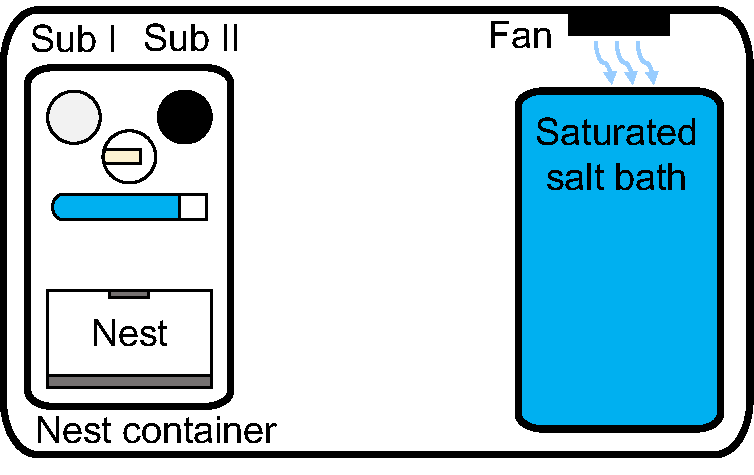
\includegraphics[width=0.75\linewidth,height=0.37\textheight]{/Users/gregchism/Library/Mobile Documents/com~apple~CloudDocs/Desktop/HumidityProject/analysis/figures/Fig1} \end{flushleft}

\textbf{Fig 1. Comparing a natural nest wall of a \emph{Temnothorax
rugatulus} colony in the field (a) and wall built by a \emph{T.
rugatulus} colony experimentally (b).} Notably, the natural nest wall is
moist and caked together, where the stone (sand) walls in the lab can
easily be pushed apart. In both photos, the outer and inner boundaries
represent the built nest wall and inside of the inner boundary is where
the queen(s), workers, and brood reside (internal nest area).

~

\textbf{\emph{Colony acclimation period}}

We first acclimated our experimental colonies in a controlled
environment produced in a climate chamber for five days (see Initial
housing and care). We determined experimental length through a
preliminary building assay, where we allowed the colonies to build nests
using experimental building substrates (see description below) for
twenty days and found no substantial nest wall changes after 10 days. We
therefore set 10 days as the building duration for our future
experimental building phases.

~

\textbf{\emph{Initial housing and care}}

During the acclimation period, we housed the colonies in 17.5cm x 12.5cm
x 6cm plastic containers with inside walls coated in `insect-a-slip'
(BioQuip product \#2871A) to prevent escape. We gave each colony a nest
space made of two glass panes (102mm x 76mm) separated by a 1.5-mm-thick
strip of cardboard at the back and smaller piece of cardboard at the
front {[}25{]}. On the opposite end of the container, we gave each
colony a water-filled 5 ml plastic tube with a cotton ball stopper and
fed each colony \emph{ad libitum} weekly with both a 2ml microcentrifuge
tube of honey water with a concentration of 1/4 teaspoon per 50ml water,
and 1/8 of a fresh-frozen cockroach (approximately 0.075g) (
\emph{Nauphoeta cinerea} ). During acclimation and between experimental
trials, we kept colonies in a climate chamber with a 12:12 h light cycle
(8 a.m. to 8 p.m.), constant temperature (approximately 20°C) and
relative humidity (approximately 20-25\%).

~

\textbf{\emph{Experimental timeline}}

We exposed each colony to one of nine humidity levels (see S1 Table). We
allowed the humidity in each container to stabilize for one day, at
which point we then provided the experimental building substrates for
colonies to build for 10 days. We photographed the colony on days 1, 5,
and 10 to determine the average number of workers and brood, but only
considered day 10 for calculating nest wall properties. We gave colonies
a 10-day rest period in ambient temperature and humidity before the
second trial in which we placed the colonies into the humidity three
places forward along the gradient (i.e.~55\% went to 85\%, and 85\% went
to 1\%).

~

\textbf{\emph{Experimental building substrates}}

We chose two distinct building substrates to allow T. rugatulus colonies
to modify their nest spaces. We offered 10g of both 1.25mm diameter
white aquarium substrate (CaribSea Super Naturals™ white aquarium
substrate: substrate I - weight of 100 pieces = 0.529g) and 0.65mm
diameter black aquarium substrate (Flourite® black sand: substrate II -
weight of 100 pieces = 0.035g) as building materials. Though substrate I
would cover more area per grain when building, its weight per grain is
15x larger than substrate II, making it harder to transport.

~

\textbf{\emph{Experimental setup}}

\textbf{Experimental nest housing}

We placed colonies in new nest sites and containers following the same
protocol as during the acclimation period (see Fig 2 for a full set
visualization).

\begin{flushleft}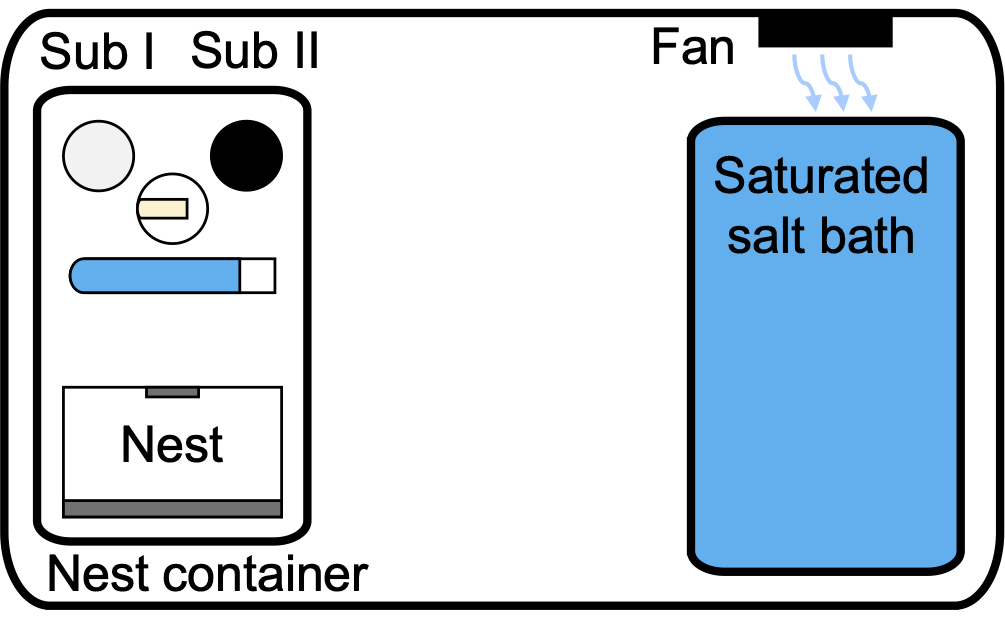
\includegraphics[width=0.75\linewidth,height=0.37\textheight]{/Users/gregchism/Library/Mobile Documents/com~apple~CloudDocs/Desktop/HumidityProject/analysis/figures/Fig2} \end{flushleft}

\textbf{Fig 2. Experimental set up for each humidity treatment.} Ants
are confined to the nest container, which contains a small pile of each
building substrate and food and water. A small fan gently circulated air
above the saturated salt water to ensure homogeneous humidity across the
system. While this system was closed (locked airtight), a small hole was
cut from the lid allowing access to the nest container to deposit each
building substrate, thus temporarily opening the system when needed.

~

\textbf{Experimental humidity levels}

For each experimental trial, we placed the nine individual colonies and
their nest containers into larger plastic containers (31.3cm x 23cm x
10.2cm). We created a discrete-step humidity gradient consisting of 9
separate boxes, each with a different, constant, regulated humidity
level. Eight of these were achieved by using saturated salt solutions,
which produce highly replicable humidity levels at 20°C in a closed,
airtight system (Fig 2; S1 Table; Winston and Bates 1960; Greenspan
1977). We used the desiccant phosphorous pentoxide to produce nearly 0\%
RH (Winston and Bates 1960). We placed each saturated salt solution and
desiccant in a plastic container (17.5cm x 12.5cm x 6cm) next to the
nest container in the experimental setup (Fig 2). We used a DC current
fan (4cm x 4cm x 4cm, 12V, 0.1A) in the top left corner of the
experimental setup to circulate air in the closed system, since
saturated salt solutions require air circulation for reproducibility
(Winston and Bates 1960). This fan was placed in the top left corner
above the saturated salt solution, angled horizontally, facing parallel
to the length of the box (Fig 2).

~

\textbf{Substrate, food, and water placement}

We inserted substrates, food, and water through a small 3.5cm hole above
the nest section, which only temporarily broke the closed, airtight
system of the colony box. We placed individual 10.0g piles of each
building substrate at the opposite end of the housing nest, such that
one substrate type was on the left and the other on the right. On day 7
of the experiment, we provided new 5ml cotton-ball-clogged water tubes,
5ml honey water microcentrifuge tubes, and 1/8 fresh-frozen cockroaches
to continue \emph{ad libitum} feeding. We randomized the arrangement of
the building substrates such that half of the colonies had the heavier
substrate on the left side and the other half on the right side (Fig 2).
During the second trial we flipped each colony's substrate placement. We
performed this procedure to prevent a side bias from affecting building
substrate choice.

~

\textbf{\emph{Data collection}}

\textbf{Environmental data}

During each experimental round, we recorded the temperature (°C) and
relative humidity (\%) of our experimental closed systems every 45
minutes using permanently imbedded U12-012 HOBO data loggers (Onset,
Bourne, MA, USA) to ensure stability and reproducibility of each section
of the relative humidity gradient (S1 Table for experimentally produced
humidity levels).

~

\textbf{Image capture and analysis}

We photographed each colony with an HD camera (Nikon D7000 with 60mm
lens). We used the image analysis software \emph{Fiji} {[}28{]} to
measure the wall length (mm), wall area (mm2), and nest area (mm2) for
every colony, which are measurement methods we derived from {[}25{]}.
Additionally, we assigned coordinates to every worker and brood item in
the nest. We standardized all measurements and coordinates from
\emph{Fiji} using the x-distance between the top left and bottom right
of the glass pane as reference points as the known distance of 102mm.

~

\textbf{Nest wall composition}

After each building period, we collected each built wall by gently
tilting a colony's housing nest space and extracting the grains while
the ants were inside the nest, allowing us to prevent panic. We sieved
the nest walls built by each colony using a 1mm colander to separate the
two substrates, and then weighed each substrate using a digital scale
(Ohaus, USA) to the nearest 0.00001g.

~

\textbf{Nest wall weight and density}

We determined wall weight by weighing the substrates each colony used to
build their nest walls. We calculated wall volume
(mm\textsuperscript{3+}) as the nest area multiplied by 1.5 mm (the
height of the provided nest cavity). We then calculated nest wall
density as total wall weight (g) / wall volume (mm\textsuperscript{3+}).

~

\textbf{Building substrate porosity}

We used the collected substrates (see colony collections) of real
\emph{T. rugatulus} nest walls to compare the porosity between natural
nests and our artificial building substrates. We allowed the substrates
to dry in open air for seven days before storing them again. Our final
sample size was 10 measures of porosity for the natural and each
experimental substrate. Porosity (Pt) is calculated by determining the
void space (Vp) in which water can fill in a substrate and dividing it
by the bulk volume (Vt) which is the void and substrate (Vs) volumes: Vt
= Vp + Vs; Pt = (Vp/Vt) x 100.

~

\textbf{Experimental substrates}

We measured the porosity of each artificial substrate by filling a 5 ml
tube with 2 ml of each substrate (total volume: Vt). We determined the
pore volume by fully saturating the substrate with deionized water
injected through a syringe to the 2 ml mark. We took water from a
container of water (weighed to the nearest 0.001g) and then determined
the volume used (Vp) by subtracting the remaining container weight from
the original weight of water. We converted water weight to volume per
the 1g/ml standard conversion for pure water. We then calculated
porosity for each substrate using the formula: Pt = (Vp/Vt) x 100.

~

\textbf{Natural nest walls}

To compare the porosities of natural and experimentally built nest
walls, we measured the porosity of natural wall substrates by filling 5
ml tubes with each natural nest's substrates and then marking where the
tube was filled. We again filled the container with deionized water from
a container of water (weighed to the nearest 0.001g) to complete
saturation at the marked substrate volume line, then we subtracted the
remaining container weight from the original weight of water to
determine the pore volume (Vp). We removed the substrates from the
containers and filled water to the line representing the volume of each
substrate and weighed that amount to the nearest 0.001g (Vt). We again
converted volume from water weight to volume per the standard 1g/ml
conversion for pure water. We then calculated porosity for each
substrate using the formula: Pt = (Vp/Vt) x 100.

~

\textbf{\emph{Final data and analysis}}

We conducted all data wrangling, analyses, and visualizations in the
software R (v4.1.1) {[}29{]} in RStudio (v1.2.5042) {[}30{]}, primarily
utilizing the tidyverse language (`tidyverse' v1.3.1) {[}31{]}. We have
made the final data and R script used for this study openly available in
a GitHub repository: https://github.com/Gchism94/HumidityProject

~

\textbf{Distance to the brood center}

We had different final sample sizes for the first (trial 1) and second
(trial 2) humidity treatments a colony experienced. We did not include
three colonies in our final trial 1 data set due to colony death (trial
1 final N = 19 colonies). Three colonies were not placed into a second
treatment since the first relative humidity produced in the first trial
was not reliable (trial 2 final N = 16).

~

\textbf{Humidity treatment analyses}

\emph{Substrate preference}: we used Mann-Whitney U tests to see whether
colonies built their walls with a preferred substrate.

~

\emph{Influence of humidity and colony size on built walls}: we took
average values for worker and brood number (see image capture and
analysis) to reduce measurement error from worker and brood occlusion in
nest containers. We used linear mixed effects models using the packages
to examine whether relative humidity or colony size influenced nest wall
feature, or internal nest area. All linear mixed effects models here and
below were conducted using the R package `lme4' (v1.1-27.1; Bates et
al., 2014), where \emph{p} values were calculated through the R package
`lmerTest' (v3.1-3; Kuznetsova et al., 2017). We found that an order
effect was present when considering a colony's first and second trial
placement, which we could not separate from the humidity treatment
placement due to unequal sample sizes (lower:higher N = 14; higher:lower
= 5). We therefore assigned the first and second trial (`Trial') as a
random effect in our models, and by comparing the variation explained by
the fixed effects alone (marginal R\textsuperscript{2+}) and with the
random effect included (conditional R\textsuperscript{2+}), we
determined the amount of variation that Trial number explained (marginal
and conditional R\textsuperscript{2+} values calculated through the R
package `MuMIn' v1.43.17; Kamil Bartoń 2020).

~

\emph{Worker and brood mortality and humidity exposure}: we first used a
linear regression to test whether brood and worker death were
correlated. We then calculated worker and brood mortality as the
proportion of average workers or brood in trial 2 over the average in
trial 1, signifying how many of each died in between trials (10 days).
We used binomial family generalized linear models to test whether the
relative mortality of workers and brood was affected by the level of
relative humidity each colony experienced in trial 1. Finally, we tested
whether colony mortality was higher in smaller or larger colonies
(average number of brood or workers) by comparing the two linear
regressions with an ANOVA: formula = log(Trial 2 colony size)
\textasciitilde{} log(Trial 1 colony size); formula = log(Trial 2 colony
size) \textasciitilde{} 1 + offset(Trial 1 colony size). The offset
function changes the model intercept to 1, where smaller colonies
experienced higher mortality with a model intercept smaller than 1 and
larger colonies experienced higher mortality with a model intercept
greater than 1.

\textbf{Building substrate porosity analysis}

We used pairwise Dunn's tests with False Discovery Rate corrected
\emph{p} values {[}35{]} to compare the median porosity of our
experimental and collected natural nest wall substrates (each N = 10).

~

\textbf{Fidelity and occurrence zone assignment}

We used the R package simr (v1.0.6) {[}36, 37{]} to calculate post hoc
power analyses for each of our linear mixed effects models where we used
0.5 and 0.8 as biologically relevant Cohen's d effect sizes (moderate
and high effect sizes) {[}38{]}. We first derived the appropriate effect
size for each model (`Humidity' fixed effect \(\beta\) coefficient) from
the formulas: Cohen's d = \(\beta\) / (sqrt(N) x SE), where N = sample
size and SE = standard error of each `Humidity' term. The simr package
determines statistical power by (i) simulating new values for the
response variable from our models; (ii) refitting our models to the
simulated response variable; (iii) applying a likelihood ratio test to
the simulated model fit. Statistical power is then determined by the
ratio of significant \emph{p} values over non-significant.

~

\textbf{\emph{Results}}

\textbf{Ants prefer small-grained substrate but show no side bias}

We used two-sided Wilcoxon tests with a predicted median value of 0.5 to
show that ants showed a substrate preference in trial 1 (W = 183,
\emph{p} \textless{} 0.001) and trial 2 (W = 132, \emph{p} \textless{}
0.001). The predominant substrate that ants used for building was the
smaller-grained substrate: in trial 1, the median weight of substrate I
that colonies used to build walls 0.160g, and 0.516g for substrate II,
with the median proportion of substrate II per substrate I being 0.746,
while in trial 2 the median grams of substrate I used was 0.011, and
0.073 substrate II, with the median proportion of substrate II per
substrate I being 0.849.

~

\textbf{Relative humidity did not influence any measured nest trait}

In our experiment, ants did not change any wall characteristics with
environmental relative humidity levels (linear mixed effects models:
wall weight - \emph{p} = 0.772; Fig 3a, S2 Table; wall length - \emph{p}
= 0.459; Fig 3b, S3 Table, wall area - \emph{p} = 0.978; Fig 4c, S4
Table, wall density - \emph{p} = 0.653; Fig 4d, S5 Table, wall substrate
composition - \emph{p} = 0.248; Fig 4e, S6 Table, internal nest area -
\emph{p} = 0.215; Fig 4f, S7 Table). `Humidity' as a fixed effect
explained little to none of the variation in the data, while random
effects did explain most of the data variation (S2-6 Tables), except for
internal nest area (S7 Table). Since we did not find an effect of
humidity on any of our measured nest traits, but our sample sizes may be
argued to be small, we ran post hoc power analyses to determine the
statistical power of each linear mixed effects model. Our models had
80\%-85.0\% power (therefore at least conventional power) {[}38{]} to
find any effects of 0.5 (mean difference, \(\beta\), divided by standard
deviation) or higher and 98\%-100\% power to find any effects of 0.8 or
higher, indicating that our negative results are likely not a
consequence of low power (S8 Table), and we can conclude that if any
effects existed they are likely to be small.

\begin{flushleft}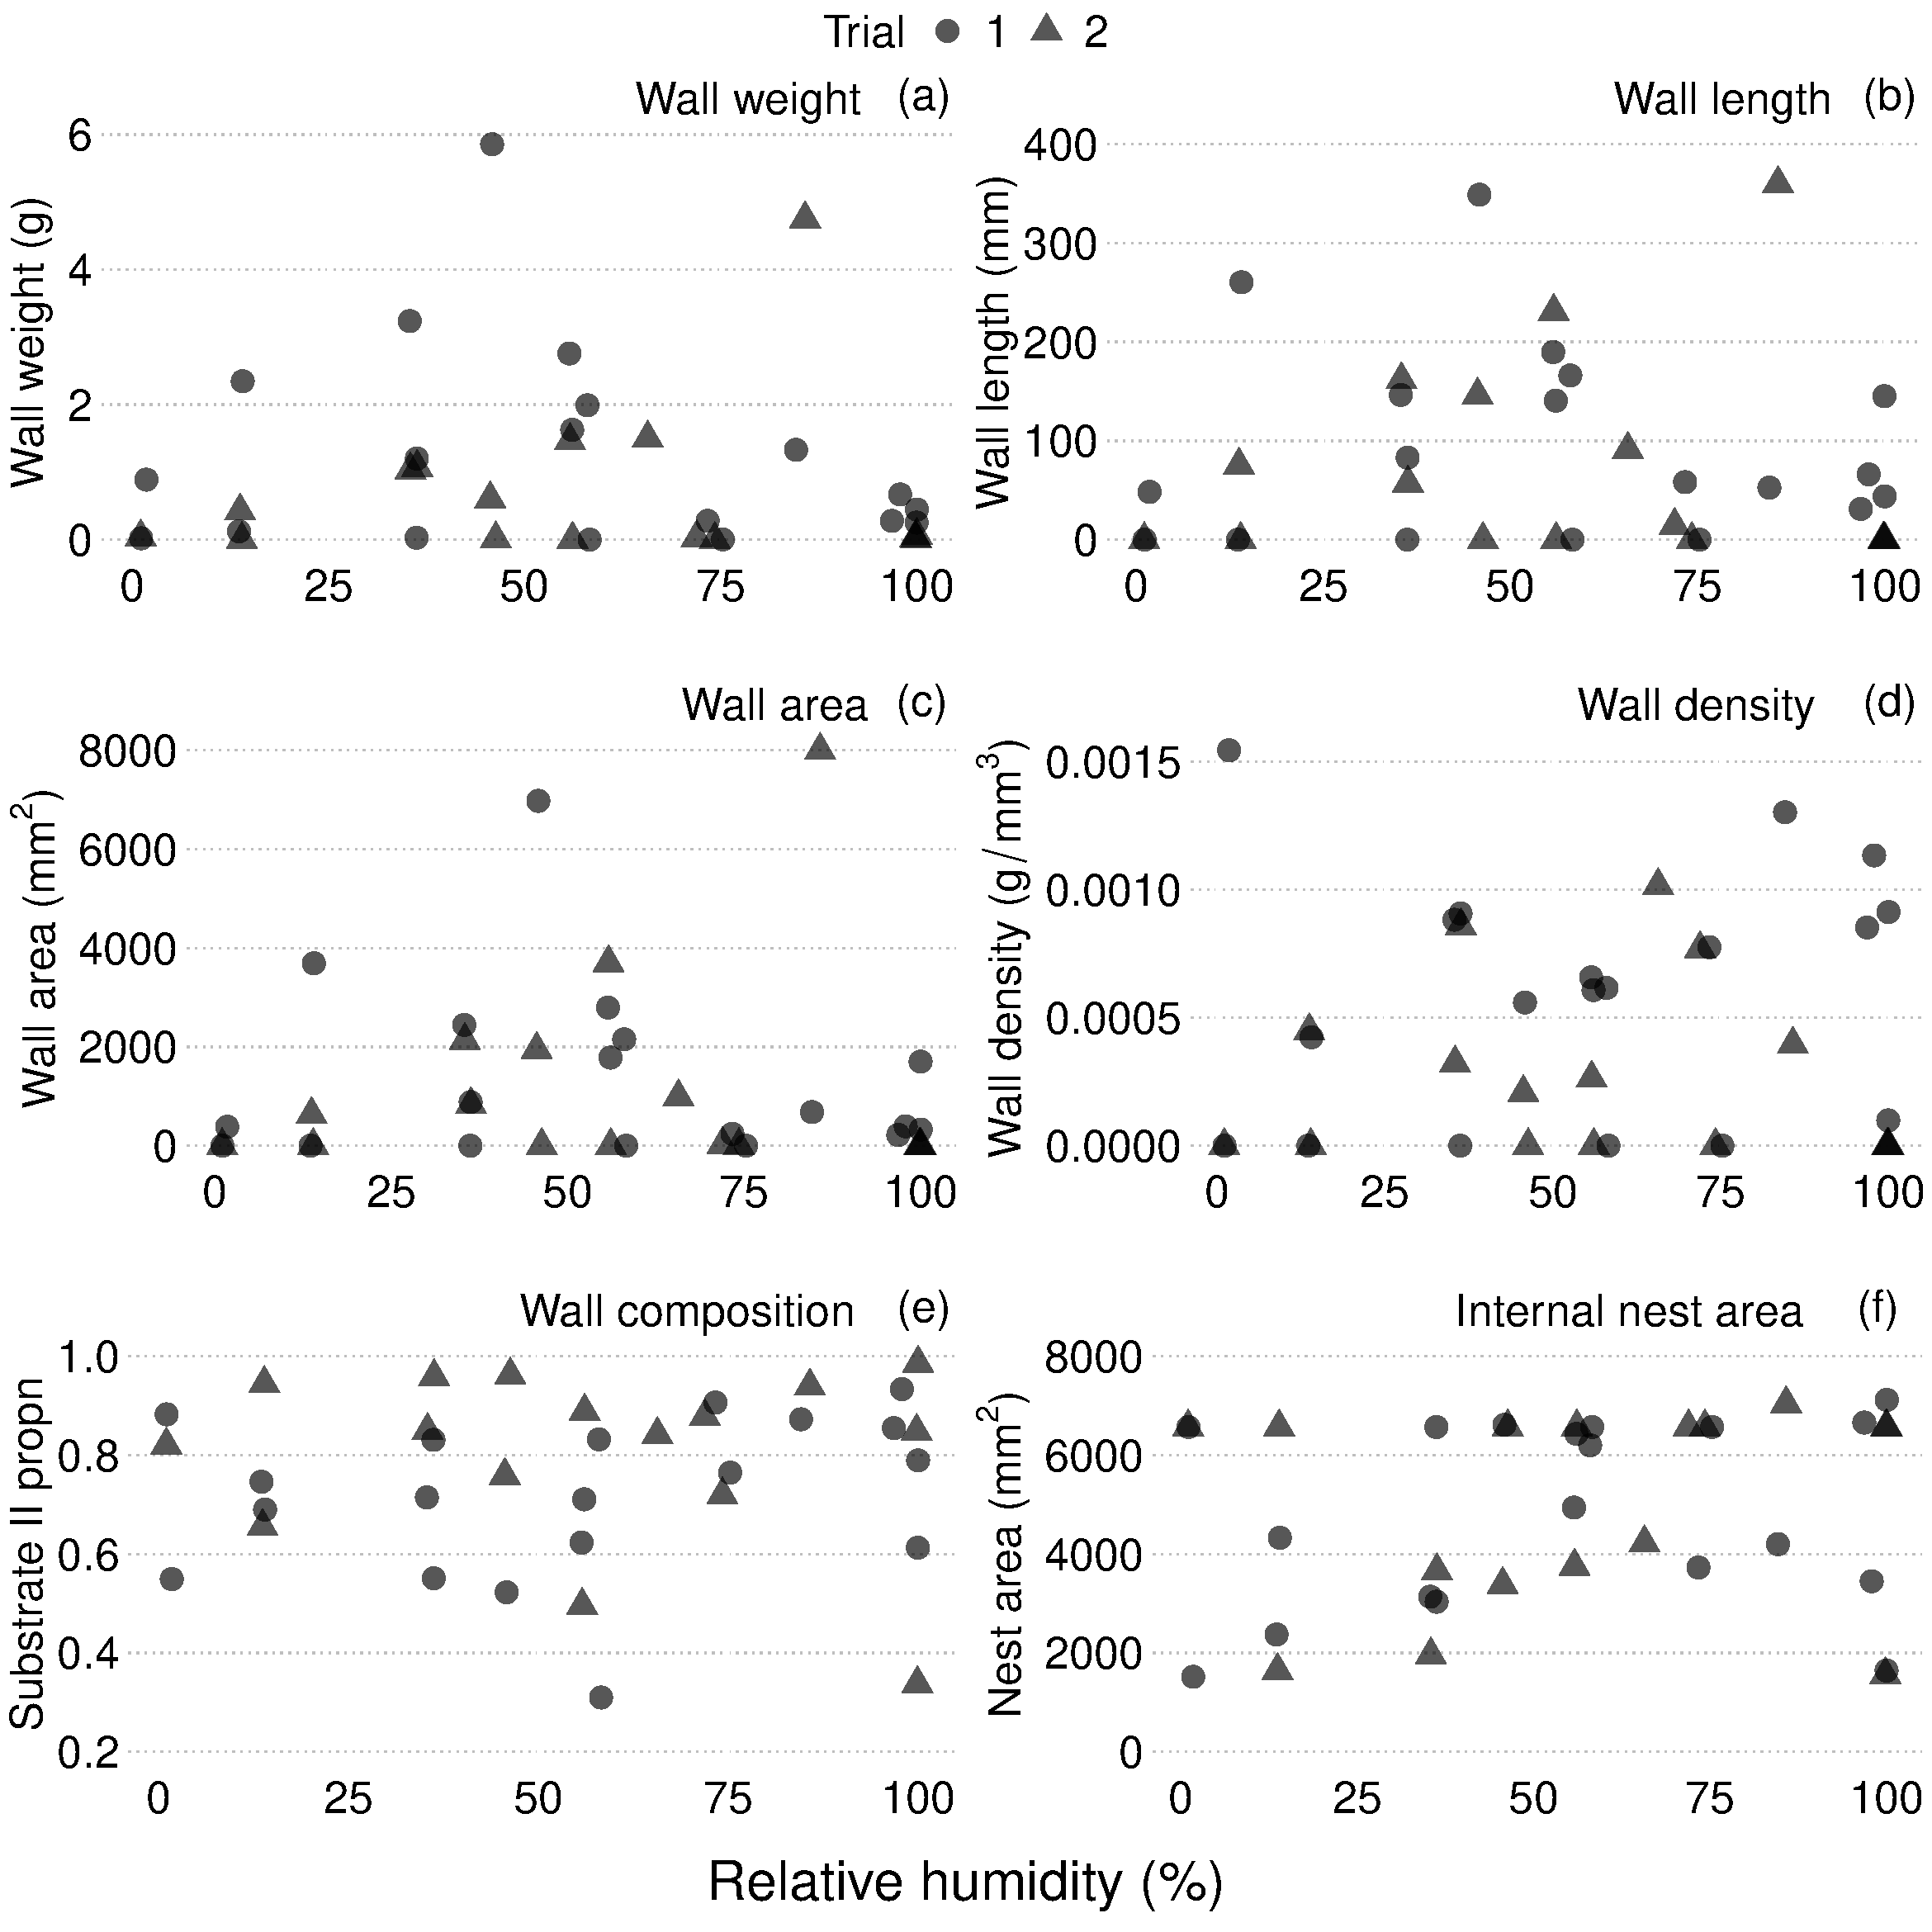
\includegraphics[width=1\linewidth,height=0.75\textheight]{/Users/gregchism/Library/Mobile Documents/com~apple~CloudDocs/Desktop/HumidityProject/analysis/figures/Fig3} \end{flushleft}

\textbf{Fig 3. The built nest wall traits measured show no relationship
with external humidity levels for trial 1 or 2.} Wall weight (a), length
(b), area (c), density (d), proportion of substrate II in nest wall (e),
and internal nest area (f). Here, and below, trial 1 data points are
circles and trial 2 are triangles.

~

\textbf{No evidence for colony size influencing nest traits}

Colonies used in our experiment varied in their demography (note that
colony size was calculated by averaging observations of workers and
brood from days 1, 5, and 10 of the experiment): the median colony size
was 84 workers in trial 1 (range 13-300; 65.3 brood items, range 2-259;
2 queens, range 1-11) and 65.5 workers in trial 2 (range 15-159; 65.7
brood items, range 11 - 190; 2 queens, range 1-11). In our experiment,
ant colony size (number of brood or workers) did not influence any wall
characteristics (linear mixed effects models: wall weight - brood:
\emph{p} = 0.275, workers: \emph{p} = 0.517; Fig 4a, S9 Table, wall
length - brood: \emph{p} = 0.054, workers: \emph{p} = 0.367; Fig 4b, S10
Table, wall area - brood: \emph{p} = 0.178, workers: \emph{p} = 0.625;
Fig 4c, S11 Table, wall density - brood: \emph{p} = 0.288, workers:
\emph{p} = 0.448; Fig 4d, S12 Table; wall substrate composition - brood:
\emph{p} = 0.622, workers: \emph{p} = 0.142; Fig 4e, S13 Table, internal
nest area - brood: \emph{p} = 0.488, workers: \emph{p} = 0.730; Fig 4f,
S14 Table). Since we did not find an effect of colony size on any of our
measured nest traits, but our sample sizes may be argued to be small, we
ran post hoc power analyses to determine the statistical power of each
linear mixed effects model. Our models had 64\%-81\% power to find any
effects of 0.5 (mean difference, \(\beta\), divided by standard
deviation) or higher and 99\%-100\% power to find any effects of 0.8 or
higher, indicating that our negative results are likely not a
consequence of low power (S15 Table). Notably, in {[}25{]} nest wall
area increasing with brood number with an effect size (calculated as we
did above) of 0.52 and our model testing for this relationship had 78\%
statistical power, so we likely had sufficient power to detect an
analogous effect.

\begin{flushleft}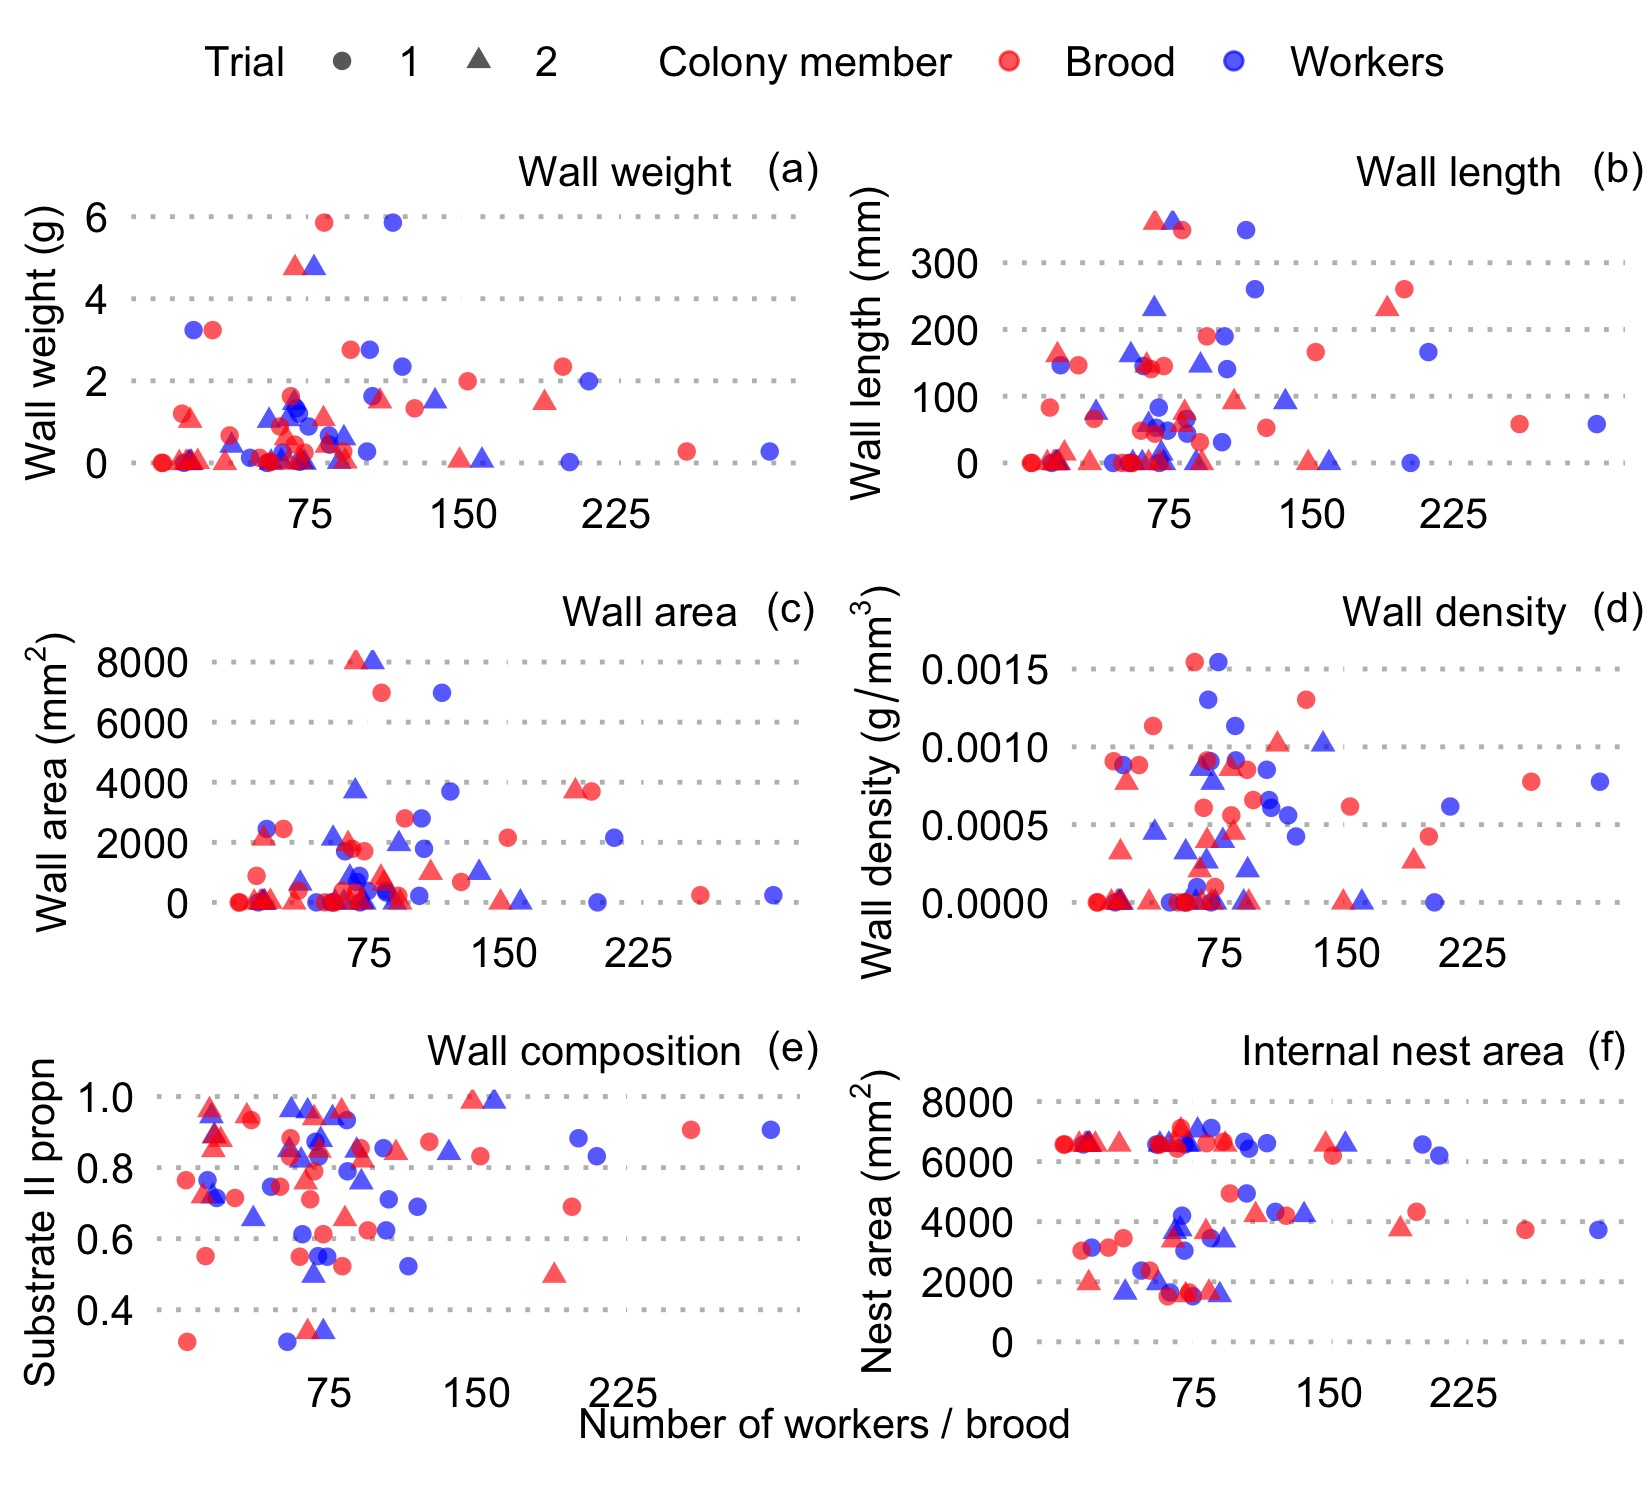
\includegraphics[width=1\linewidth,height=0.75\textheight]{/Users/gregchism/Library/Mobile Documents/com~apple~CloudDocs/Desktop/HumidityProject/analysis/figures/Fig4} \end{flushleft}

\textbf{Fig 4. The built nest wall traits measured show no relationship
with the number of brood (blue) or workers (red) in a colony for trial 1
or 2.} Wall weight (a), length (b), area (c), density (d), proportion of
substrate II in nest wall (e), and internal nest area (f).

~

\textbf{Colony mortality did not relate to relative humidity, but larger
colonies had higher mortality } We found that worker and brood mortality
was highly correlated (\(\beta\) = 1.042 ± 0.168, \emph{p} \textless{}
0.001; S1 Fig, S16 Table). We however found no relationship between
relative humidity and the proportion of colony member deaths between
trials (10-days) in our generalized linear models (Workers: \emph{p} =
0.694; Brood: \emph{p} = 0.756; S2 Fig, S17 Table). We lastly found that
the slopes in our linear models predicting colony size in trial 2 from
trial 1 were less than 1 (S2 Fig, S18 Table) and were significantly
different than models with a slope of 1 (ANOVA: Brood: \emph{F} = 8.47,
\emph{p} = 0.021; Workers: \emph{F} = 6.79, \emph{p} = 0.011; S19
Table). Slopes smaller than 1 indicate that mortality was lower in
larger colonies, but since there was no correlation with humidity, the
cause is likely not desiccation from low relative humidity or disease
(e.g.~fungal infection) from high relative humidity.

~

\textbf{Colonies preferred the more porous building substrate, which
resembled natural nest walls}

We found that ants prefer a more porous substrate: substrate I, the one
with smaller grains and thus lower porosity, was not preferred; and in
fact, the walls built in our experiment had similar porosity to natural
walls collected in the field (\emph{Z} = 154, \emph{p} = 0.077), as well
as being similar to pure substrate II (\emph{Z} = 134, \emph{p} = 0.345)
(Fig 5, S20 Table). However, the natural wall substrate was likely not
as compact in our porosity assays as in nature, which could possibly
change the results. In natural walls, substrate appears tamped down,
whereas it was loosely shaken into the test vial for our porosity
assays.

\begin{flushleft}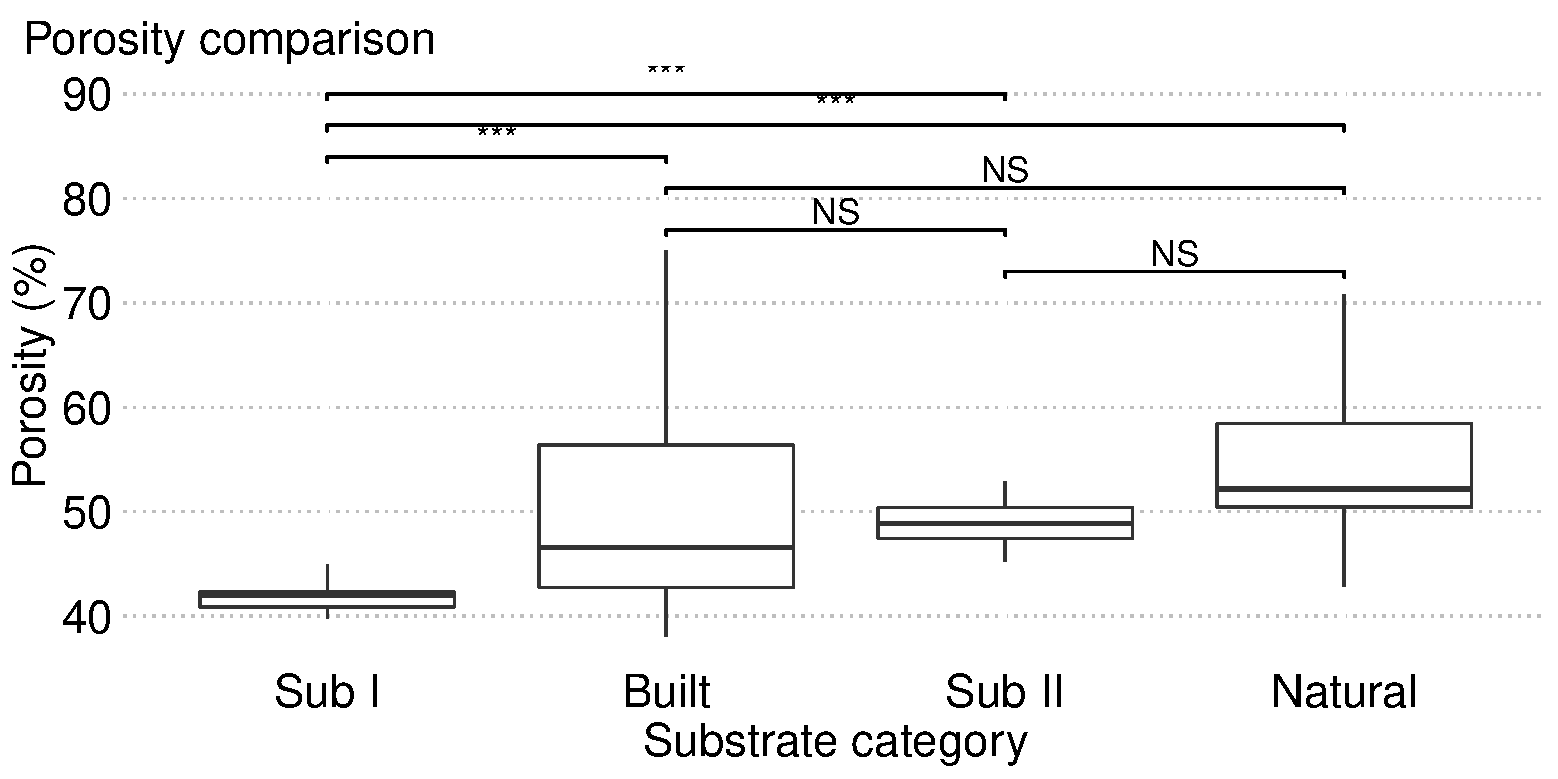
\includegraphics[width=0.67\linewidth,height=0.5\textheight]{/Users/gregchism/Library/Mobile Documents/com~apple~CloudDocs/Desktop/HumidityProject/analysis/figures/Fig5} \end{flushleft}

\textbf{Fig 5. Comparison of porosity between the artificial and natural
\emph{Temnothorax rugatulus} nest wall substrates.} Bars denote sample
medians, boxes represent the first and third quantiles, lines denote the
data range. Stars denote significant Dunn's pairwise multiple
comparisons tests.

~

\textbf{\emph{Discussion}}

Our study does not support the hypothesis that environmental humidity
affects nest building in \emph{Temnothorax rugatulus}. We found no
influence of external humidity on any measured nest property (Fig 3).
This might indicate that the nest wall properties are not under
selection for maintaining a certain humidity level inside the nest
space, or that if they are, they are not plastic (ants do not flexibly
adapt them to changing needs for insulation from the environment). We
also did not find the effect reported in {[}25{]}, that nest wall area
scales up with brood number in a colony (Fig 4), nor did any other nest
property increase with colony size (Fig 4). This inconsistency could
stem from different experimental designs -- the authors in {[}25{]}
considered low and high humidity while our study had nine humidity
levels - or from the low statistical power of our study. We additionally
did not find a relationship between the first relative humidity level
that colonies experienced in our study and worker or brood mortality; we
did find that larger colonies had overall higher relative mortality
(S1-2 Figs). We lastly saw that both our small experimental substrate
(substrate II) and the built experimental walls are significantly more
porous than the larger experimental substrate but had similar porosity
to natural \emph{T. rugatulus} built nest walls. This may be because
ants are aiming for porous walls, or it may result from a preference for
carrying larger sand grains (which may make the building process more
efficient) {[}23{]}.

Humidity regulation is only one function of social insect nests;
however, the internal humidity of the nest can be so important that
social insects build structural modifications towards its strict
regulation. Examples of these structures include ventilation turrets and
thatched nests in \emph{Atta leafcutter} ants {[}11, 12, 39, 40{]} and
thicker, reinforced mounds along the east-to-west nest axes of
\emph{Macrotermes} termites towards retaining water in the nest
{[}13-15{]}. Here we show in contrast that environmental humidity does
not influence \emph{Temnothorax rugatulus} nest wall structure inside
nest cavities, suggesting that humidity regulation is not a function of
\emph{Temnothorax} nests. Indeed, intrinsic (genetics) rather than
extrinsic (temperature and humidity) factors are shown to be more
influential towards the nest architectures that harvester ants build
{[}41{]}. In addition, our \emph{T. rugatulus} colonies selected a less
energetically expensive substrate to build with (substrate II),
consistent with previous work on wall building substrate choice in
\emph{Temnothorax albipennis} colonies {[}22{]}. Changing built nest
walls in response to humidity might be energetically expensive, which
may constrain the flexibility that \emph{T. rugatulus} has in regulating
in-nest humidity through wall composition. Additionally, in the desert,
external humidity and temperature can change quickly and thus plastic
adjustment of nest walls may not be possible, leading to ants building a
nest wall structure that is suitable at all levels of humidity.
Alternatively, humidity may not be regulated in \emph{T. rugatulus}
nests, but instead are physiologically resistant to varying
environmental humidity. Instead, \emph{T. rugatulus} colonies may
consider other purposes such as nest defense or regulating worker
interactions through changing nest densities.

Our study confirms that the spatial distribution of colony members in
ant nests is not identical to one that would be produced by `random
movement'. We do not propose that it is realistic that ants move
randomly; rather, we believe this is an appropriate null hypothesis to
clarify whether the outcome of movement is in fact different from one in
which individual actions do not add up to a non-random trend to
accumulate in particular areas. In other studies, the outcome of ant
movement has sometimes been indistinguishable from similar null
hypotheses of randomness (e.g.~worker sorting: Sendova-Franks and Van
Lent 2002; interactions between potential and returning foragers:
Davidson and Gordon 2017). Additionally, movement in the nest from one
ant \emph{T. albipennis} can be predicted by movement from another, and
faster movement occurs when more ants are in motion (Gallotti and
Chialvo 2018). Outside of the nest, random movement that is reinforced
by trail pheromones explains ant coordination along specific trails to
and from food sources and the nest (Ma et al., 2013; Chang et al.,
2021). The non-random nest occupation of our \emph{T. rugatulus}
colonies therefore demonstrates not only that individual ants' movement
is not random, but that in aggregate, individual movement rules are such
that they bias worker movement to produce clustering and heterogeneity
in distribution at the colony level, and that the effects of nest shape
we find here cannot be produced by passive effects of geometry on random
movement.

The total area available in an enclosed ant nest will determine worker
density. Both nest area and worker density in the nest have previously
been demonstrated to be important in ants, and our results support this.
Nest area is an important consideration for nest site selection in
\emph{Temnothorax} ants (Pratt and Pierce 2001; Mitrus 2015), where
workers measure the size of prospective nests (Pratt 2005). Crowded
nests can significantly increase worker energy expenditure in \emph{T.
rugatulus} colonies (Cao and Dornhaus 2008), while also both increasing
foraging and scouting rates and inducing polydomy (Cao 2013). The
consequences of nest density to ant colonies, such as traffic jammed
panicked nest evacuation, can be mediated by small structural features
at the nest entrance (Burd et al., 2010; Shiwakoti et al., 2014; Wang
and Song 2016). Ants may even adaptively regulate contact rate with each
other, as a part of strategies for task allocation and information
exchange (Pacala et al., 1996; Pinter-Wollman et al., 2012;
Pinter-Wollman et al., 2013; Lehue et al., 2020b). Contact rate may also
be used to estimate colony or group size (Gordon et al., 1992; Pratt
2005; Dornhaus and Franks 2006). In our study here, we compared colonies
at two different worker densities, but also found that local density in
nests is heterogeneous and may be driven by overall nest shape and thus
access to all parts of the nest. We saw that colony members spread out
more in both nest shapes at low worker density, but this effect was more
pronounced in the tube nest shape; in addition, we saw that constraints
of space led to higher local density near the entrance in the tube nest
(e.g.~see Figs. 3-4). Our study did not address whether the spatial
distribution of colony members in their nests is a passive effect of
particular cavity shapes and densities, or a result of adaptive,
flexible individual strategies used by \emph{Temnothorax} ants in
response to the particular nest spaces encountered. \emph{Temnothorax}
ants, in nature, can also modify their nest spaces by adding internal
stone walls to the cavity their nest inhabits (Franks et al., 1992;
Franks and Deneubourg 1997; Aleksiev et al., 2007a; Aleksiev et al.,
2007b; Aleksiev et al., 2007c; DiRienzo and Dornhaus 2017). The purpose
of such nest modifications is not well studied, but it is a possibility
that these ants actively modify either the available area or the shape
of their nest space. Future work may reveal more about how these spatial
distributions affect colony performance, and thus spatial properties of
both nest cavities and colony distribution matter most to colonies.

The innate internal humidity of nest cavities may be an important
consideration for \emph{Temnothorax} nest site selection.
\emph{Temnothorax} ants demonstrate extensive decision-making in
house-hunting {[}42-46{]}, which relates several properties in potential
nest cavities. For example, emigrating colonies determine nest size
through interactions with other exploring nest mates (quorum sensing)
{[}47{]}. Also, nest cavities that have smaller nest entrances {[}44,
48{]} are more sought after by \emph{Temnothorax} ants for properties
such as less light invasion {[}48{]}. Additionally, rock-dwelling
\emph{Temnothorax albipennis} colonies have been shown to remove
substrate from new nest cavities in relation to worker density in the
nest (i.e.~nest `molting') {[}27{]}, posing an alternative mechanism
that may also regulate in-nest humidity. Therefore, either innate nest
cavity properties, or alternative mechanisms to nest wall building, may
produce a desirable humidity inside of the nest space (i.e.~rock
crevices), where \emph{Temnothorax} ants do not need to build nest walls
towards its regulation.

Our study is also the first to consider the porosity of the natural and
artificial substrates used by \emph{Temnothorax} ants for wall building.
Porosity, i.e.~the amount of void space between the packed substrate,
may influence nest properties in a variety of ways, including
thermoregulation and moisture retention, as well as costs of building
per volume of wall, none of which has been well studied so far in
\emph{Temnothorax} ants. In addition, the soil available to
\emph{Temnothorax} ants in nature likely exhibits a variety of
properties that don't exist in grains of sand, such as the ability to
retain moisture in extremely small soil and cellulose grain sizes. The
natural nest walls of \emph{Temnothorax rugatulus} ants can be very
densely packed which translated to very slow water penetration in our
porosity assays when compared to the virtually instantaneous water
penetration of our experimental walls. The mud-brick-like natural
\emph{T. rugatulus} nest walls (GC personal observation, but also see
Fig 1) may therefore trap humidity differently than loosely packed stone
walls. A separate experiment would test this by providing substrates
with a variety of weights, types, and sizes could allow rock dwelling
ants to select material that produces more compact nest walls than
previously possible in both ours and past studies {[}22, 23, 25{]}.
Alternatively, \emph{Temnothorax} ants may just build with what is
available and produce walls with a random mix of substrates that are
more energetically efficient to build and those that retain more
moisture. Notably, colonies of the ponerine ant \emph{Rhytidoponera
metallica} also dwell in rocks and build nest modifications from
environmental substrates {[}49, 50{]}, and other rock dwelling ants
differ in their nest size preference {[}50{]}. We suggest that exploring
the traits of substrates that rock-dwelling ants build nest walls with
will provide greater insight to the purpose of these nest walls.

\hypertarget{acknowledgements}{%
\section{Acknowledgements}\label{acknowledgements}}

\begin{enumerate}
\def\labelenumi{\arabic{enumi}.}
\item
  Wilson EO, Kinne O. Success and dominance in ecosystems: the case of
  the social insects. Oldendorf/Luhe: Ecology Institute; 1990. Available
  From: https://www.int-res.com/articles/eebooks/eebook02.pdf
\item
  Jeanne RL. The adaptiveness of social wasp nest architecture. Q Rev
  Biol. 1975 Sep;50(3):267-87. doi: https://doi.org/10.1086/408564
\item
  Seeley TD, Seeley RH, Akratanakul P. Colony defense strategies of the
  honeybees in Thailand. Ecol Monogr. 1982 Mar;52(1):43-63. doi:
  10.2307/2937344
\item
  Tschinkel WR. Seasonal life history and nest architecture of a
  winter-active ant, Prenolepis imparis. Insectes Soc. 1987
  Sep;34(3):143-64. doi: https://doi.org/10.1007/BF02224081
\item
  London KB, Jeanne RL. The interaction between mode of colony founding,
  nest architecture and ant defense in polistine wasps. Ethol Ecol Evol.
  2000 Mar;12(1):13-25. doi:
  https://doi.org/10.1080/03949370.2000.9728440
\item
  Tschinkel WR. The nest architecture of the ant, Camponotus socius. J
  Insect Sci. 2005 Jan;5(1):9. doi: https://doi.org/10.1093/jis/5.1.9
\item
  Tschinkel WR. The nest architecture of three species of north Florida
  Aphaenogaster ants. J Insect Sci. 2011 Jan;11(1):105. doi:
  https://doi.org/10.1673/031.011.10501
\item
  Pinter-Wollman N. Nest architecture shapes the collective behaviour of
  harvester ants. Biol Lett. 2015 Oct;11(10):20150695. doi:
  https://doi.org/10.1098/rsbl.2015.0695
\item
  Wilson EO. The ergonomics of caste in the social insects. Am Nat. 1968
  Jan;102(923):41-66. doi: https://doi.org/10.1086/282522
\item
  Hansell M. Animal architecture. 1st edition. Oxford University Press
  on Demand; 2005. doi:
  https://doi.org/10.1093/acprof:oso/9780198507529.001.0001
\item
  Bollazzi M, Roces F. To build or not to build: circulating dry air
  organizes collective building for climate control in the leaf-cutting
  ant Acromyrmex ambiguus. Anim Behav. 2007 Nov;74(5):1349-1355. doi:
  https://doi.org/10.1016/j.anbehav.2007.02.021
\item
  Bollazzi M, Roces F. Leaf-cutting ant workers (Acromyrmex heyeri)
  trade off nest thermoregulation for humidity control. J Ethol. 2010
  May;28(2):399-403. doi: https://doi.org/10.1007/s10164-010-0207-3
\item
  Noirot C, Darlington JP. Termite nests: architecture, regulation and
  defence. Termites: evolution, sociality, symbioses, ecology.
  Dordrecht: Springer; 2000:121-139. doi:
  https://doi.org/10.1007/978-94-017-3223-9\_6
\item
  Korb J. Thermoregulation and ventilation of termite mounds.
  Naturwissenschaften. 2003 May;90(5):212-9. doi:
  https://doi.org/10.1007/s00114-002-0401-4
\item
  Korb J. Termite mound architecture, from function to construction.
  Biology of termites: a modern synthesis. Dordrecht: Springer;
  2010:349-373. doi: https://doi.org/10.1007/978-90-481-3977-4\_13
\item
  Brian MV, Hibble J, Stradling DJ. Ant pattern and density in a
  southern English heath. The J Anim Ecol. 1965 Oct;1:545-55. doi:
  10.2307/2448
\item
  Coenen-staß D. Investigations on the water balance in the red wood
  ant, Formica polyctena (Hymenoptera, Formicidae): workers, their
  larvae and pupae. Comp Biochem Physiol A Physiol. 1986
  Jan;83(1):141-7. doi: https://doi.org/10.1016/0300-9629(86)90101-5
\item
  North RD. Transpiration and humidity preference in a temperate wood
  ant Formica rufa L. J Insect Physiol. 1991 Jan;37(4):279-86. doi:
  https://doi.org/10.1016/0022-1910(91)90062-5
\item
  Bengston SE. Life-history and behavioral trait covariation across 3
  years in Temnothorax ants. Behav Ecol. 2018 Nov;29(6):1494-1501. doi:
  https://doi.org/10.1093/beheco/ary101
\item
  Franks NR, Wilby A, Silverman BW, Tofts C. Self-organizing nest
  construction in ants: sophisticated building by blind bulldozing. Anim
  behav. 1992 Aug;44:357-75. doi:
  https://doi.org/10.1016/0003-3472(92)90041-7
\item
  Franks NR, Deneubourg JL. Self-organizing nest construction in ants:
  individual worker behaviour and the nest's dynamics. Anim Behav. 1997
  Oct;54(4):779-96. doi: https://doi.org/10.1016/0003-3472(92)90041-7
\item
  Aleksiev AS, Longdon B, Christmas MJ, Sendova-Franks, AB, Franks NR.
  Individual choice of building material for nest construction by worker
  ants and the collective outcome for their colony. Anim Behav. 2007
  Sep;74(3):559-566. doi: hhttps://doi.org/10.1016/j.anbehav.2006.12.019
\item
  Aleksiev AS, Sendova-Franks AB, Franks NR. The selection of building
  material for wall construction by ants. Anim Behav. 2007 May;73(5),
  779-788. doi: https://doi.org/10.1016/j.anbehav.2006.06.014
\item
  Aleksiev AS, Sendova-Franks AB, Franks NR. Nest `moulting' in the ant
  Temnothorax albipennis. Anim Behav. 2007 Sep;74(3), 567-575. doi:
  https://doi.org/10.1016/j.anbehav.2006.12.023
\item
  DiRienzo N, Dornhaus A. Temnothorax rugatulus ant colonies
  consistently vary in nest structure across time and context. PLoS One.
  2017 Jun;12(6):e0177598. doi:
  https://doi.org/10.1371/journal.pone.0177598
\item
  Winston PW, Bates DH. Saturated solutions for the control of humidity
  in biological research. Ecology. 1960 Jan;41(1):232-7. doi:
  10.2307/1931961
\item
  Greenspan L. Humidity fixed points of binary saturated aqueous
  solutions. J Res Natl Bur Stand A Phys Chem. 1977 Jan;81(1):89. doi:
  10.6028/jres.081A.011
\item
  Schindelin J, Arganda-Carreras I, Frise E, Kaynig V, Longair M,
  Pietzsch T, et al.~Fiji: an open-source platform for biological-image
  analysis. Nat Methods. 2012 Jul;9(7):676-82. doi:
  https://doi.org/10.1038/nmeth.2019
\item
  Team RC. R: A language and environment for statistical computing.
  Available From: URL https://www.R-project.org/.
\item
  Allaire J. RStudio: integrated development environment for R. Boston,
  MA. 2012;770(394):165-71. Available From: http://www.rstudio.com/.
\item
  Wickham H, Averick M, Bryan J, Chang W, McGowan LD, François R, et
  al.~Welcome to the Tidyverse. J Open Source Softw. 2019 Nov
  21;4(43):1686. doi: 10.21105/joss.01686
\item
  Bates D, Mächler M, Bolker B, Walker S. Fitting linear mixed-effects
  models using lme4. arXiv:1406.5823 {[}Preprint{]}. 2014 {[}cited 2022
  May 18{]}. Available from: https://doi.org/10.18637/jss.v067.i01
\item
  Kuznetsova A, Brockhoff PB, Christensen RH. lmerTest package: tests in
  linear mixed effects models. J Stat Softw. 2017 Dec;82:1-26. doi:
  https://doi.org/10.18637/jss.v082.i13
\item
  Bartoń K. MuMIn: Multi-Model Inference. R package version 1.43.17.
  2022. Available From: https://CRAN.R-project.org/package=MuMIn
\item
  Benjamini Y, Hochberg Y. Controlling the false discovery rate: a
  practical and powerful approach to multiple testing. J R Stat Soc
  Series B Stat Methodol. 1995 Jan;57(1):289-300. doi:
  https://doi.org/10.1111/j.2517-6161.1995.tb02031.x
\item
  Champely S, Ekstrom C, Dalgaard P, Gill J, Weibelzahl S, Anandkumar A,
  et al.~pwr: Basic Functions for Power Analysis. R package version
  1.3-0. 2017. Available From: https://CRAN.R-project.org/package=pwr
\item
  Green P, MacLeod CJ. SIMR: an R package for power analysis of
  generalized linear mixed models by simulation. Methods Ecol Evol. 2016
  Apr;7(4):493-8. doi: https://doi.org/10.1111/2041-210X.12504
\item
  Cohen J. Statistical power analysis for the behavioral sciences. 2nd
  ed.~New York: Routledge; 2013. doi: 10.4324/9780203771587
\item
  Roces F, Kleineidam C. Humidity preference for fungus culturing by
  workers of the leaf-cutting ant Atta sexdens rubropilosa. Insectes
  Soc. 2000 Nov;47(4):348-50. doi: https://doi.org/10.1007/PL00001728
\item
  Halboth F, Roces F. The construction of ventilation turrets in Atta
  vollenweideri leaf-cutting ants: Carbon dioxide levels in the nest
  tunnels, but not airflow or air humidity, influence turret structure.
  PLoS One. 2017 Nov;12(11):e0188162. doi:
  https://doi.org/10.1371/journal.pone.0188162
\item
  O'Fallon S, Lowell ES, Daniels D, Pinter-Wollman N. Harvester ant nest
  architecture is more strongly affected by intrinsic than extrinsic
  factors. Behav Ecol. 2022 May;33(3):644-53. doi:
  https://doi.org/10.1093/beheco/arac026
\item
  Dornhaus A, Franks NR, Hawkins RM, Shere HN. Ants move to improve:
  colonies of Leptothorax albipennis emigrate whenever they find a
  superior nest site. Anim Behav. 2004 May;67(5):959-63. doi:
  https://doi.org/10.1016/j.anbehav.2003.09.004
\item
  Franks NR, Pratt SC, Mallon EB, Britton NF, Sumpter DJ. Information
  flow, opinion polling and collective intelligence in house--hunting
  social insects. Proc R Soc Lond B Biol Sci. 2002
  Nov;357(1427):1567-83. doi: https://doi.org/10.1098/rstb.2002.1066
\item
  Franks NR, Dornhaus A, Metherell BG, Nelson TR, Lanfear SA, Symes WS.
  Not everything that counts can be counted: ants use multiple metrics
  for a single nest trait. Proc R Soc Lond B Biol Sci. 2006
  Jan;273(1583):165-9. doi: https://doi.org/10.1098/rspb.2005.3312
\item
  Sasaki T, Pratt SC. Ants learn to rely on more informative attributes
  during decision-making. Biol Lett. 2013 Dec;9(6):20130667. doi:
  https://doi.org/10.1098/rsbl.2013.0667
\item
  Sasaki T, Colling B, Sonnenschein A, Boggess MM, Pratt SC. Flexibility
  of collective decision making during house hunting in Temnothorax
  ants. Behav Ecol Sociobiol. 2015 May;69(5):707-14. doi:
  https://doi.org/10.1007/s00265-015-1882-4
\item
  Pratt SC. Quorum sensing by encounter rates in the ant Temnothorax
  albipennis. Behav Ecol. 2005 Mar;16(2):488-96. doi:
  https://doi.org/10.1093/beheco/ari020
\item
  Pratt SC, Pierce NE. The cavity-dwelling ant Leptothorax curvispinosus
  uses nest geometry to discriminate between potential homes. Anim
  Behav. 2001 Aug;62(2):281-7. doi:
  https://doi.org/10.1006/anbe.2001.1777
\item
  Robinson WA. Selection and sharing of sheltered nest sites by ants
  (Hymenoptera: Formicidae) in grasslands of the Australian Capital
  Territory. Aust J Entomol. 2008 Aug;47(3):174-83. doi:
  https://doi.org/10.1111/j.1440-6055.2008.00632.x
\item
  Thomas ML. Nest site selection and longevity in the ponerine ant
  Rhytidoponera metallica (Hymenoptera, Formicidae). Insectes Soc. 2002
  May;49(2):147-52. doi: https://doi.org/10.1007/s00040-002-8294-y
\end{enumerate}

\hypertarget{supporting-information}{%
\section{Supporting information}\label{supporting-information}}

\textbf{S1 Fig. Percentage of brood and worker death in each colony
after trial 1 shows no relationship with external humidity levels.}

\textbf{S2 Fig. Relatively fewer brood and workers died in larger
colonies during the experiment.} Points are the average brood or
workers, black lines denote a slope of 1 and red lines are slopes
derived from linear models (e.g., formula: log(BroodTrial2)
\textasciitilde{} log(BroodTrial1)).

\textbf{S1 Table. Predicted and empirical levels of relative humidity
(\%) produced from saturated salt solutions.} Predicted relative
humidity levels (mean ± standard deviation) are in 20 - 25°C and
empirical in 20.40°C ± 0.18°C. Note that magnesium acetate was not used
in trial 2 because it produced an inconsistent RH \% in trial 1.

\textbf{S2 Table. Relationship between built nest wall weight (g) and
relative humidity (\%).} Linear mixed effects model: WallWt
\textasciitilde{} Humidity + (1 \textbar{} Trial)

\textbf{S3 Table. Relationship between built nest wall length (mm) and
relative humidity (\%) for each experimental trial.} Linear mixed
effects model: Length \textasciitilde{} Humidity + (1 \textbar{} Trial)

\textbf{S4 Table. Relationship between built nest wall area (mm2) and
relative humidity (\%) for each experimental trial.} Linear mixed
effects model: Area \textasciitilde{} Humidity + (1 \textbar{} Trial)

\textbf{S5 Table. Relationship between built nest wall density (g/mm3)
and relative humidity (\%) for each experimental trial.} Linear mixed
effects model: Density \textasciitilde{} Humidity + (1 \textbar{} Trial)

\textbf{S6 Table. Relationship between the wall substrate composition
(proportion of substrate II in build walls) and relative humidity (\%)
for each experimental trial.} Linear mixed effects model: PropIIWall
\textasciitilde{} Humidity + (1 \textbar{} Trial)

\textbf{S7 Table. Relationship between the internal nest area (mm2) and
relative humidity (\%) for each experimental trial.} Linear mixed
effects model: Nest.Area \textasciitilde{} Humidity + (1 \textbar{}
Trial)

\textbf{S8 Table. Statistical power analyses of linear mixed effects
models assessing the effect of humidity on nest properties.} Power
analyses considered a moderate (Cohen's d = 0.5) and high (Cohen's d =
0.8) effect size. The direction of the effect was taken from the
corresponding linear mixed effects model.

\textbf{S9 Table. Relationship between built nest wall weight (g) and
colony size (number of brood and workers).} Linear mixed effects model:
CollWallWt \textasciitilde{} Number.Colony + (1 \textbar{} Trial)

\textbf{S10 Table. Relationship between built nest wall length (mm) and
colony size (number of brood and workers).} Linear mixed effects model:
Length \textasciitilde{} Number.Colony + (1 \textbar{} Trial)

\textbf{S11 Table. Relationship between built nest wall area (mm2) and
colony size (number of brood and workers).} Linear mixed effects model:
Area \textasciitilde{} Number.Colony + (1 \textbar{} Trial)

\textbf{S12 Table. Relationship between built nest wall density (g/mm3)
and colony size (number of brood and workers).} Linear mixed effects
model: Density \textasciitilde{} Number.Colony + (1 \textbar{} Trial)

\textbf{S13 Table. Relationship between built nest wall composition
(proportion of substrate II) and colony size (number of brood and
workers).} Linear mixed effects model: PropIIWall \textasciitilde{}
Number.Colony + (1 \textbar{} Trial)

\textbf{S14 Table. Relationship between internal nest area (mm2) and
colony size (number of brood and workers).} Linear mixed effects model:
Nest.Area \textasciitilde{} Number.Colony + (1 \textbar{} Trial)

\textbf{S15 Table. Statistical power of our linear mixed effects models
assessing the effect of colony size on nest properties.} Power analyses
considered a moderate (Cohen's d = 0.5) and high (Cohen's d = 0.8)
effect size. The direction of the effect was taken from the
corresponding linear mixed effects model.

\textbf{S16 Table. Relationship between brood and worker mortality (\%)
after trial 1.} Linear regression: Brood.Death \textasciitilde{}
Worker.Death

\textbf{S17 Table. Relationship between the percentage of worker and
brood death in a colony (\%) and relative humidity (\%).} The percent
death was taken after the first experimental trial. Generalized linear
model: worker or brood death \textasciitilde{} Humidity, family =
Binomial

\textbf{S18 Table. Relationship between the log of average brood or
workers in trials 1 and 2.} Linear regression: Model 1 = Formula:
log(avg.worker Trial 2) \textasciitilde{} log(avg.worker Trial 1); Model
2 = Formula: log(avg.brood Trial2) \textasciitilde{} 1+
offset(log(avg.brood Trial1))

\textbf{S19 Table. Comparing linear models from Table S18 to models with
an intercept of 1.} Model comparison: ANOVA(Model 1 \textasciitilde{}
Model 2); Model 1 = Formula: log(avg.worker Trial 2) \textasciitilde{}
log(avg.worker Trial 1); Model 2 = Formula: log(avg.brood Trial2)
\textasciitilde{} 1+ offset(log(avg.brood Trial1))

\textbf{S20 Table. Comparing the artificial and natural wall substrates
porosities (\%).} Dunn's pairwise tests for wall substrate types:
Porosity \textasciitilde{} SubstrateType


\end{document}
